\documentclass{beamer}

\usetheme{Warsaw}
\usepackage{graphicx}
\usepackage{ulem}
\usepackage{tikz}
\usetikzlibrary{shapes,arrows}
\usepackage{subcaption}
\usepackage{algorithm,algorithmic}
\usepackage{natbib}
\usepackage{cancel}
% include.tex
\newcommand{\Bernoulli}[1]{\text{Bernoulli} \left( #1 \right)}
\newcommand{\mydigamma}[1]{\psi \left( #1 \right)}
%\newcommand{\diag}[1]{\text{diag}\left( #1 \right)}
\newcommand{\tr}[1]{\text{tr}\left( #1 \right)}
\newcommand{\Poisson}[1]{\text{Poisson} \left( #1 \right)}
\def \half {\frac{1}{2}}
\def \R {\mathbb{R}}
\def \vbeta {\vec{\beta}}
\def \vy {\vec{y}}
\def \vmu {\vec{\mu}}
\def \vmuqbeta {\vmu_{q(\vbeta)}}
\def \vmubeta {\vmu_{\vbeta}}
\def \Sigmaqbeta {\Sigma_{q(\vbeta)}}
\def \Sigmabeta {\Sigma_{\vbeta}}
\def \va {\vec{a}}
\def \vtheta {\vec{\theta}}
\def \mX {\vec{X}}

\def\ds{{\displaystyle}}

\def\diag{{\mbox{diag}}}


\usepackage{latexsym,amssymb,amsmath,amsfonts}
%\usepackage{tabularx}
\usepackage{theorem}
\usepackage{verbatim,array,multicol,palatino}
\usepackage{graphicx}
\usepackage{graphics}
\usepackage{fancyhdr}
\usepackage{algorithm,algorithmic}
\usepackage{url}
%\usepackage[all]{xy}



\def\approxdist{\stackrel{{\tiny \mbox{approx.}}}{\sim}}
\def\smhalf{\textstyle{\frac{1}{2}}}
\def\vxnew{\vx_{\mbox{{\tiny new}}}}
\def\bib{\vskip12pt\par\noindent\hangindent=1 true cm\hangafter=1}
\def\jump{\vskip3mm\noindent}
\def\etal{{\em et al.}}
\def\etahat{{\widehat\eta}}
\def\thick#1{\hbox{\rlap{$#1$}\kern0.25pt\rlap{$#1$}\kern0.25pt$#1$}}
\def\smbbeta{{\thick{\scriptstyle{\beta}}}}
\def\smbtheta{{\thick{\scriptstyle{\theta}}}}
\def\smbu{{\thick{\scriptstyle{\rm u}}}}
\def\smbzero{{\thick{\scriptstyle{0}}}}
\def\boxit#1{\begin{center}\fbox{#1}\end{center}}
\def\lboxit#1{\vbox{\hrule\hbox{\vrule\kern6pt
      \vbox{\kern6pt#1\kern6pt}\kern6pt\vrule}\hrule}}
\def\thickboxit#1{\vbox{{\hrule height 1mm}\hbox{{\vrule width 1mm}\kern6pt
          \vbox{\kern6pt#1\kern6pt}\kern6pt{\vrule width 1mm}}
               {\hrule height 1mm}}}


%\sloppy
%\usepackage{geometry}
%\geometry{verbose,a4paper,tmargin=20mm,bmargin=20mm,lmargin=40mm,rmargin=20mm}


%%%%%%%%%%%%%%%%%%%%%%%%%%%%%%%%%%%%%%%%%%%%%%%%%%%%%%%%%%%%%%%%%%%%%%%%%%%%%%%%
%
% Some convenience definitions
%
% \bf      -> vector
% \sf      -> matrix
% \mathcal -> sets or statistical
% \mathbb  -> fields or statistical
%
%%%%%%%%%%%%%%%%%%%%%%%%%%%%%%%%%%%%%%%%%%%%%%%%%%%%%%%%%%%%%%%%%%%%%%%%%%%%%%%%

% Sets or statistical values
\def\sI{{\mathcal I}}                            % Current Index set
\def\sJ{{\mathcal J}}                            % Select Index set
\def\sL{{\mathcal L}}                            % Likelihood
\def\sl{{\ell}}                                  % Log-likelihood
\def\sN{{\mathcal N}}                            
\def\sS{{\mathcal S}}                            
\def\sP{{\mathcal P}}                            
\def\sQ{{\mathcal Q}}                            
\def\sB{{\mathcal B}}                            
\def\sD{{\mathcal D}}                            
\def\sT{{\mathcal T}}
\def\sE{{\mathcal E}}                            
\def\sF{{\mathcal F}}                            
\def\sC{{\mathcal C}}                            
\def\sO{{\mathcal O}}                            
\def\sH{{\mathcal H}} 
\def\sR{{\mathcal R}}                            
\def\sJ{{\mathcal J}}                            
\def\sCP{{\mathcal CP}}                            
\def\sX{{\mathcal X}}                            
\def\sA{{\mathcal A}} 
\def\sZ{{\mathcal Z}}                            
\def\sM{{\mathcal M}}                            
\def\sK{{\mathcal K}}     
\def\sG{{\mathcal G}}                         
\def\sY{{\mathcal Y}}                         
\def\sU{{\mathcal U}}  


\def\sIG{{\mathcal IG}}                            


\def\cD{{\sf D}}
\def\cH{{\sf H}}
\def\cI{{\sf I}}

% Vectors
\def\vectorfontone{\bf}
\def\vectorfonttwo{\boldsymbol}
\def\va{{\vectorfontone a}}                      %
\def\vb{{\vectorfontone b}}                      %
\def\vc{{\vectorfontone c}}                      %
\def\vd{{\vectorfontone d}}                      %
\def\ve{{\vectorfontone e}}                      %
\def\vf{{\vectorfontone f}}                      %
\def\vg{{\vectorfontone g}}                      %
\def\vh{{\vectorfontone h}}                      %
\def\vi{{\vectorfontone i}}                      %
\def\vj{{\vectorfontone j}}                      %
\def\vk{{\vectorfontone k}}                      %
\def\vl{{\vectorfontone l}}                      %
\def\vm{{\vectorfontone m}}                      % number of basis functions
\def\vn{{\vectorfontone n}}                      % number of training samples
\def\vo{{\vectorfontone o}}                      %
\def\vp{{\vectorfontone p}}                      % number of unpenalized coefficients
\def\vq{{\vectorfontone q}}                      % number of penalized coefficients
\def\vr{{\vectorfontone r}}                      %
\def\vs{{\vectorfontone s}}                      %
\def\vt{{\vectorfontone t}}                      %
\def\vu{{\vectorfontone u}}                      % Penalized coefficients
\def\vv{{\vectorfontone v}}                      %
\def\vw{{\vectorfontone w}}                      %
\def\vx{{\vectorfontone x}}                      % Covariates/Predictors
\def\vy{{\vectorfontone y}}                      % Targets/Labels
\def\vz{{\vectorfontone z}}                      %

\def\vone{{\vectorfontone 1}}
\def\vzero{{\vectorfontone 0}}

\def\valpha{{\vectorfonttwo \alpha}}             %
\def\vbeta{{\vectorfonttwo \beta}}               % Unpenalized coefficients
\def\vgamma{{\vectorfonttwo \gamma}}             %
\def\vdelta{{\vectorfonttwo \delta}}             %
\def\vepsilon{{\vectorfonttwo \epsilon}}         %
\def\vvarepsilon{{\vectorfonttwo \varepsilon}}   % Vector of errors
\def\vzeta{{\vectorfonttwo \zeta}}               %
\def\veta{{\vectorfonttwo \eta}}                 % Vector of natural parameters
\def\vtheta{{\vectorfonttwo \theta}}             % Vector of combined coefficients
\def\vvartheta{{\vectorfonttwo \vartheta}}       %
\def\viota{{\vectorfonttwo \iota}}               %
\def\vkappa{{\vectorfonttwo \kappa}}             %
\def\vlambda{{\vectorfonttwo \lambda}}           % Vector of smoothing parameters
\def\vmu{{\vectorfonttwo \mu}}                   % Vector of means
\def\vnu{{\vectorfonttwo \nu}}                   %
\def\vxi{{\vectorfonttwo \xi}}                   %
\def\vpi{{\vectorfonttwo \pi}}                   %
\def\vvarpi{{\vectorfonttwo \varpi}}             %
\def\vrho{{\vectorfonttwo \rho}}                 %
\def\vvarrho{{\vectorfonttwo \varrho}}           %
\def\vsigma{{\vectorfonttwo \sigma}}             %
\def\vvarsigma{{\vectorfonttwo \varsigma}}       %
\def\vtau{{\vectorfonttwo \tau}}                 %
\def\vupsilon{{\vectorfonttwo \upsilon}}         %
\def\vphi{{\vectorfonttwo \phi}}                 %
\def\vvarphi{{\vectorfonttwo \varphi}}           %
\def\vchi{{\vectorfonttwo \chi}}                 %
\def\vpsi{{\vectorfonttwo \psi}}                 %
\def\vomega{{\vectorfonttwo \omega}}             %


% Matrices
%\def\matrixfontone{\sf}
%\def\matrixfonttwo{\sf}
\def\matrixfontone{\bf}
\def\matrixfonttwo{\boldsymbol}
\def\mA{{\matrixfontone A}}                      %
\def\mB{{\matrixfontone B}}                      %
\def\mC{{\matrixfontone C}}                      % Combined Design Matrix
\def\mD{{\matrixfontone D}}                      % Penalty Matrix for \vu_J
\def\mE{{\matrixfontone E}}                      %
\def\mF{{\matrixfontone F}}                      %
\def\mG{{\matrixfontone G}}                      % Penalty Matrix for \vu
\def\mH{{\matrixfontone H}}                      %
\def\mI{{\matrixfontone I}}                      % Identity Matrix
\def\mJ{{\matrixfontone J}}                      %
\def\mK{{\matrixfontone K}}                      %
\def\mL{{\matrixfontone L}}                      % Lower bound
\def\mM{{\matrixfontone M}}                      %
\def\mN{{\matrixfontone N}}                      %
\def\mO{{\matrixfontone O}}                      %
\def\mP{{\matrixfontone P}}                      %
\def\mQ{{\matrixfontone Q}}                      %
\def\mR{{\matrixfontone R}}                      %
\def\mS{{\matrixfontone S}}                      %
\def\mT{{\matrixfontone T}}                      %
\def\mU{{\matrixfontone U}}                      % Upper bound
\def\mV{{\matrixfontone V}}                      %
\def\mW{{\matrixfontone W}}                      % Variance Matrix i.e. diag(b'')
\def\mX{{\matrixfontone X}}                      % Unpenalized Design Matrix/Nullspace Matrix
\def\mY{{\matrixfontone Y}}                      %
\def\mZ{{\matrixfontone Z}}                      % Penalized Design Matrix/Kernel Space Matrix

\def\mGamma{{\matrixfonttwo \Gamma}}             %
\def\mDelta{{\matrixfonttwo \Delta}}             %
\def\mTheta{{\matrixfonttwo \Theta}}             %
\def\mLambda{{\matrixfonttwo \Lambda}}           % Penalty Matrix for \vnu
\def\mXi{{\matrixfonttwo \Xi}}                   %
\def\mPi{{\matrixfonttwo \Pi}}                   %
\def\mSigma{{\matrixfonttwo \Sigma}}             %
\def\mUpsilon{{\matrixfonttwo \Upsilon}}         %
\def\mPhi{{\matrixfonttwo \Phi}}                 %
\def\mOmega{{\matrixfonttwo \Omega}}             %
\def\mPsi{{\matrixfonttwo \Psi}}                 %

\def\mone{{\matrixfontone 1}}
\def\mzero{{\matrixfontone 0}}

% Fields or Statistical
\def\bE{{\mathbb E}}                             % Expectation
\def\bP{{\mathbb P}}                             % Probability
\def\bR{{\mathbb R}}                             % Reals
\def\bI{{\mathbb I}}                             % Reals
\def\bV{{\mathbb V}}                             % Reals

\def\vX{{\vectorfontone X}}                      % Targets/Labels
\def\vY{{\vectorfontone Y}}                      % Targets/Labels
\def\vZ{{\vectorfontone Z}}                      %

% Other
\def\etal{{\em et al.}}
\def\ds{\displaystyle}
\def\d{\partial}
\def\diag{\text{diag}}
%\def\span{\text{span}}
\def\blockdiag{\text{blockdiag}}
\def\tr{\text{tr}}
\def\RSS{\text{RSS}}
\def\df{\text{df}}
\def\GCV{\text{GCV}}
\def\AIC{\text{AIC}}
\def\MLC{\text{MLC}}
\def\mAIC{\text{mAIC}}
\def\cAIC{\text{cAIC}}
\def\rank{\text{rank}}
\def\MASE{\text{MASE}}
\def\SMSE{\text{SASE}}
\def\sign{\text{sign}}
\def\card{\text{card}}
\def\notexp{\text{notexp}}
\def\ASE{\text{ASE}}
\def\ML{\text{ML}}
\def\nullity{\text{nullity}}

\def\logexpit{\text{logexpit}}
\def\logit{\mbox{logit}}
\def\dg{\mbox{dg}}

\def\Bern{\mbox{Bernoulli}}
\def\sBernoulli{\mbox{Bernoulli}}
\def\sGamma{\mbox{Gamma}}
\def\sInvN{\mbox{Inv}\sN}
\def\sNegBin{\sN\sB}

\def\dGamma{\mbox{Gamma}}
\def\dInvGam{\mbox{Inv}\Gamma}

\def\Cov{\mbox{Cov}}
\def\Mgf{\mbox{Mgf}}

\def\mis{{mis}} 
\def\obs{{obs}}

\def\argmax{\operatornamewithlimits{\text{argmax}}}
\def\argmin{\operatornamewithlimits{\text{argmin}}}
\def\argsup{\operatornamewithlimits{\text{argsup}}}
\def\arginf{\operatornamewithlimits{\text{arginf}}}


\def\minimize{\operatornamewithlimits{\text{minimize}}}
\def\maximize{\operatornamewithlimits{\text{maximize}}}
\def\suchthat{\text{such that}}


\def\relstack#1#2{\mathop{#1}\limits_{#2}}
\def\sfrac#1#2{{\textstyle{\frac{#1}{#2}}}}


\def\comment#1{
\vspace{0.5cm}
\noindent \begin{tabular}{|p{14cm}|}  
\hline #1 \\ 
\hline 
\end{tabular}
\vspace{0.5cm}
}


\def\mytext#1{\begin{tabular}{p{13cm}}#1\end{tabular}}
\def\mytextB#1{\begin{tabular}{p{7.5cm}}#1\end{tabular}}
\def\mytextC#1{\begin{tabular}{p{12cm}}#1\end{tabular}}

\def\jump{\vskip3mm\noindent}

\def\KL{\text{KL}}
\def\N{\text{N}}
\def\Var{\text{Var}}

\def \E {\mathbb{E}}
\def \BigO {\text{O}}
\def \IG {\text{IG}}
\def \Beta {\text{Beta}}



\usefonttheme{serif}

\title{Bayesian linear model selection}
\author{Mark Greenaway, Dr John Ormerod}

\mode<presentation>
{ \usetheme{boxes} }


\begin{document}
% 1. Front slide
\begin{frame}
	\titlepage
	% Details about myself here?
\end{frame}
			
% Only have ten minutes
% Introduce problem
\begin{frame}
	\frametitle{Posterior parameters in Bayesian linear model selection}
	\begin{itemize}
		\item Motivation: The problem of selecting linear models is well-studied, in the frequentist and Bayesian
					contexts.
		\item A lot of work has been done on parameter priors for Bayesian model selection.
		\item Less work has been done on the parameter posteriors, so we chose to explore this area in our
					research.
		\item We derive several new exact closed form expressions for the posterior parameters using special
					functions. Our expressions are numerically stable.
	\end{itemize}

\end{frame}

\begin{frame}
	\frametitle{Notation}
	\begin{itemize}
		\item Let $\vy$ be the vector of responses of length $n$, and $\mX$ be the $n \times p$ covariate matrix.
		\item We seek the best model $\vgamma$, a vector of length $p$ where
					\[
						\vgamma_i =
						\begin{cases}
							1 & \text{ if the $i$th column of $\mX$ is included in the model} \\
							0 & \text{otherwise}
						\end{cases}
					\]
		e.g. $\vgamma = (1, 0, 0, 1, 1)$ includes the first, fourth and fifth covariates from $\mX$.
		\item Then $\mX_\vgamma$ is the matrix formed by taking the columns for which $\vgamma_i = 1$ from X,
					and $p_\vgamma$ is the number of covariates in the model $\vgamma$.
	\end{itemize}
\end{frame}

% Introduce model
\begin{frame}
	\frametitle{Model selection using $g$}
	\begin{itemize}
		\item Consider the linear model
		\begin{align*}
			\vy | \alpha, \vbeta, \sigma^2, \vgamma \sim \N_n(\vone_n \alpha + \mX_\vgamma \vbeta, \sigma^2 \mI) 
		\end{align*}
		with priors
		\begin{align*}
			\alpha \quad & \propto \quad 1, \\
			\vbeta | \sigma^2, g, \vgamma \quad & \sim \quad \N_p(\vzero, g \sigma^2 (\mX_\vgamma^\top \mX_\vgamma)^{-1}),                     \\
			p(\sigma^2)          \quad & = \quad (\sigma^2)^{-1} \I(\sigma^2 > 0), \text{ and }                    \\
			p(g)                 \quad & = \quad \text{unspecified for now}.
		\end{align*}
		\item We introduce a hyperparameter $g \in [0, \infty)$, as a shrinkage parameter.
					$g$ shrinks $\vbeta$ according to the sample size $n$, the number of covariates in the model $p_\vgamma$
					and the quality of the model fit $R^2_\vgamma$.
					$g$ deserves special consideration.
		\item This prior structure on $\vbeta$ is called the Zellner-Siow prior, introduced in \cite{Zellner1980}.
		% that controls the mixing between the null and full models.
		% \item If $g$ is $0$, we
		% choose the null model. If $g$ is $\infty$ we choose $\hat{\vbeta}$.
	\end{itemize}
\end{frame}

% Discuss Bartlett's and Information Paradox
\begin{frame}
	\frametitle{How should we choose $g$?}
	There are a few approaches we could take.
	\begin{itemize}
		\item Approach 1: We could simply let $g \to \infty$.
		\item \cite{Liang2008} showed that\\
		$p(\vgamma = \vzero | \vy) \to 1$ as $g \to \infty$ (Bartlett's paradox).
		\item Approach 2: We could do Empirical Bayes on $g$, or otherwise make a fixed choice of $g$.
		\item \cite{Liang2008} showed that this was not model selection consistent. \\
					$p(\vgamma = \vgamma^* | \vy) \cancel{\to} 1$ as $n \to \infty$,
					where $\vgamma^*$ is the true model (Information Paradox)
		\item So we need another approach.
	\end{itemize}

\end{frame}

% Mixture of g, choice of g prior
\begin{frame}
	\frametitle{We should choose a mixture of $g$}
	\cite{Liang2008} argued that we avoid should these paradoxes by using a mixture of $g$. \\
	Several choices of prior for $g$	have been proposed.
	\small
	\begin{itemize}
		\item hyper-$g$ prior, \cite{Liang2008}\\
		$p(g) = \frac{a-2}{2} (1 + g)^{-a/2} I(g > 0)$, $a > 2$
		\item hyper-$g/n$ prior, \cite{Liang2008}\\
		$p(g) = \frac{a-2}{2n} (1 + g/n)^{-a/2} I(g > 0)$, $a > 2$ 
		\item Bayarri's robust prior on $g$, \cite{Bayarri2012} \\
		$p(g) = \frac{1}{2} \left(  \frac{1 + n}{1 + p_\vgamma} \right)^{1/2} (1 + g)^{-3/2} I(g > (1 + n)/(1 + p_\vgamma) - 1)$
		\item Beta-Prime prior on $g$, \cite{Maruyama2011} \\
		$p(g) = \frac{g^b (1 + g)^{-(a + b + 2)}}{\Beta(a + 1, b + 1)} \I(g > 0)$
	\end{itemize}
\end{frame}

% Things we derived
\begin{frame}
	\frametitle{Calculating $p(\vy | \vgamma)$}
	We want to calculate $p(\vy | \vgamma)$ so that we can calculate $p(\vgamma | \vy)$ using Bayes' Rule and rank models against	one another. \\
	To do this, we need to calculate
	$$p(\vy | \vgamma) = \int p(\vy | \alpha, \vbeta, \sigma^2, \vgamma) p(\alpha) p(\vbeta | g, \vgamma) p(\sigma^2) p(g) d \alpha d \vbeta d \sigma^2 d g.$$
	We choose our priors so that this integral is tractable, with help from \cite{Gradshteyn1988}.
	The marginal likelihoods behave like BIC. \\
	We found the following closed form expressions.
	\small
	\begin{itemize}
		\item Liang et al. 2008 hyper-$g$ prior \cite{Liang2008}
			$p(\vy | \vgamma) = \frac{K(n) (a - 2)}{p_\vgamma + a  - 2} {}_2 F_1 \left( \frac{n-1}{2}, 1; \frac{p_\vgamma + a}{2}; R_\vgamma^2 \right)$
		\item Liang et al. 2008 hyper-$g/n$ prior \cite{Liang2008}
			$p(\vy | \vgamma) = \frac{K(n) (a - 2)}{n (p_\vgamma + a  - 2)} F_1 \left( 1, \frac{a}{2}, \frac{n-1}{2}; \frac{p_\vgamma + a}{2}; 1 - \frac{1}{n}, R_\vgamma^2 \right)$
	\end{itemize}
	These expressions are numerically stable to evaluate.
\end{frame}

\begin{frame}
	\frametitle{Calculating $p(\vy | \vgamma)$ for Bayarri's robust prior}
	\begin{itemize}
		\item Bayarri calculated the marginal likelihood given $\vgamma$ for the Robust Bayarri prior
		 	in \cite{Bayarri2012} 
			\tiny
			$p(\vy | \vgamma) = K(n) \left(\frac{n + 1}{1 + p_\vgamma}\right)^{-p_\vgamma/2} \frac{(1 - R^2_\vgamma)^{-(n-1)/2}}{p_\vgamma + 1} {}_2 F_1 \left[ \frac{n-1}{2}, \frac{p_\vgamma+1}{2}; \frac{p_\vgamma + 3}{2}; \frac{[1 - 1/(1 - R^2_\vgamma)](p_\vgamma + 1)}{1 + n} \right]$.
		\small
		\item But this expression is not numerically well-behaved, because the second argument of the
					${}_2 F_1$ function is greater than $1$.
		\item Using Euler's transformation on ${}_2 F_1$ and the fact that ${}_2 F_1(., 1; .; .)$ is numerically
					well-behaved, we derived the new expression
			\tiny
			$p(\vy | \vgamma) = K(n) \left(\frac{n + 1}{1 + p_\vgamma}\right)^{(n-p_\vgamma-1)/2} \frac{[1 + L (1 - R^2_\vgamma)]^{-(n-1)/2}}{p_\vgamma + 1} {}_2 F_1 \left[ \frac{n-1}{2}, 1; \frac{p_\vgamma + 3}{2}; 
			\frac{R^2_\vgamma}{1 + L(1 - R^2_\vgamma)} \right]$ \\
			\small
			where $L = (1 + n)/(1 + p_\vgamma) - 1$.

	\end{itemize}
\end{frame}

% Exact posterior distributions using special functions
\begin{frame}
	\frametitle{Exact posterior distributions of $\alpha$, $u$ and $\sigma^2$ using special functions}
	When deriving exact posterior distributions on the parameters of the model,
	we focused on the Beta-Prime prior on $g$, as it is the most numerically well-behaved. \\
	We were able to derive closed form expressions for the posterior distributions.
	\small
	\begin{align*}
		p(u | \vy) &= \frac{(1 - R_\vgamma^2)^{b + 1}}{\text{Beta}(b + 1, d + 1)} u^b (1 - u)^d (1 - u R_\vgamma^2)^{-(b + d + 2)} \\
		p(\alpha | \vy) &= \frac{\Gamma(c + \frac{1}{2}) (1 - R_\vgamma^2)^{b + 1}}{\Gamma(c) \sqrt{\pi}} (1 + \alpha^2)^{-n/2}
		{}_2 F_1 \left(b + 1, c + \frac{1}{2}; c; \frac{R_\vgamma^2}{1 + \alpha^2}\right) \\
		p(\sigma^2 | \vy) &= \frac{\frac{n}{2} (1 - R_\vgamma^2)^{b + 1}}{\Gamma(c)} (1 - R_\vgamma^2)^{-(c + 1)}
												\exp{\left( -\frac{n}{2 \sigma^2} \right)} {}_1 F_1 \left(b + 1; c; \frac{n R_\vgamma^2}{2 \sigma^2}\right)
	\end{align*}
	where $u = g/(1 + g)$, $a = 1$ and $b = p_\vgamma$.
\end{frame}

\begin{frame}
	\frametitle{Exact first and second moments of $\vbeta$}
	% We weren't able to find a closed form expression for $\vbeta | \vy$, but 
	We weren't able to find a closed form expression for $\vbeta | \vy$, but we were able to find closed form
	expressions for the first and second moments of $\vbeta | \vy$.
	\small
	\begin{align*}
		\E[\vbeta | \vy] &= M_1 \hat{\vbeta} \\
		\Cov[\vbeta | \vy] &= \frac{n}{n - 3} (M_1 - M_2 R^2)(\mX^\top \mX)^{-1} + (M_2 - M_1^2) \hat{\vbeta} \hat{\vbeta}^\top
	\end{align*}
	where
	\small
	\begin{align*}
		M_1 &= \frac{b + 1}{c} {}_2 F_1 (d + 1, 1; c + 1; R^2) \text{ and } \\
		M_2 &= \frac{(b + 1)(b + 2)}{c(c + 1)} {}_2 F_1 (d + 1, 2; c + 2; R^2).
	\end{align*}
\end{frame}

% Say sopmething about the Rao-Blackwellisation?

% Graphs of posterior functions
\begin{frame}
	\frametitle{Comparing exact results to Monte Carlo sampling}
	We checked our results by comparing against Monte Carlo sampling and found that they matched closely.
	\begin{figure}[htp]
		\centering
		\begin{center}$
			\begin{array}{ll}
				% \caption{$u | \vy$}
				\includegraphics[width=.5\textwidth]{uGivenY.pdf} &
				% \caption{$\sigma^2 | \vy$}
				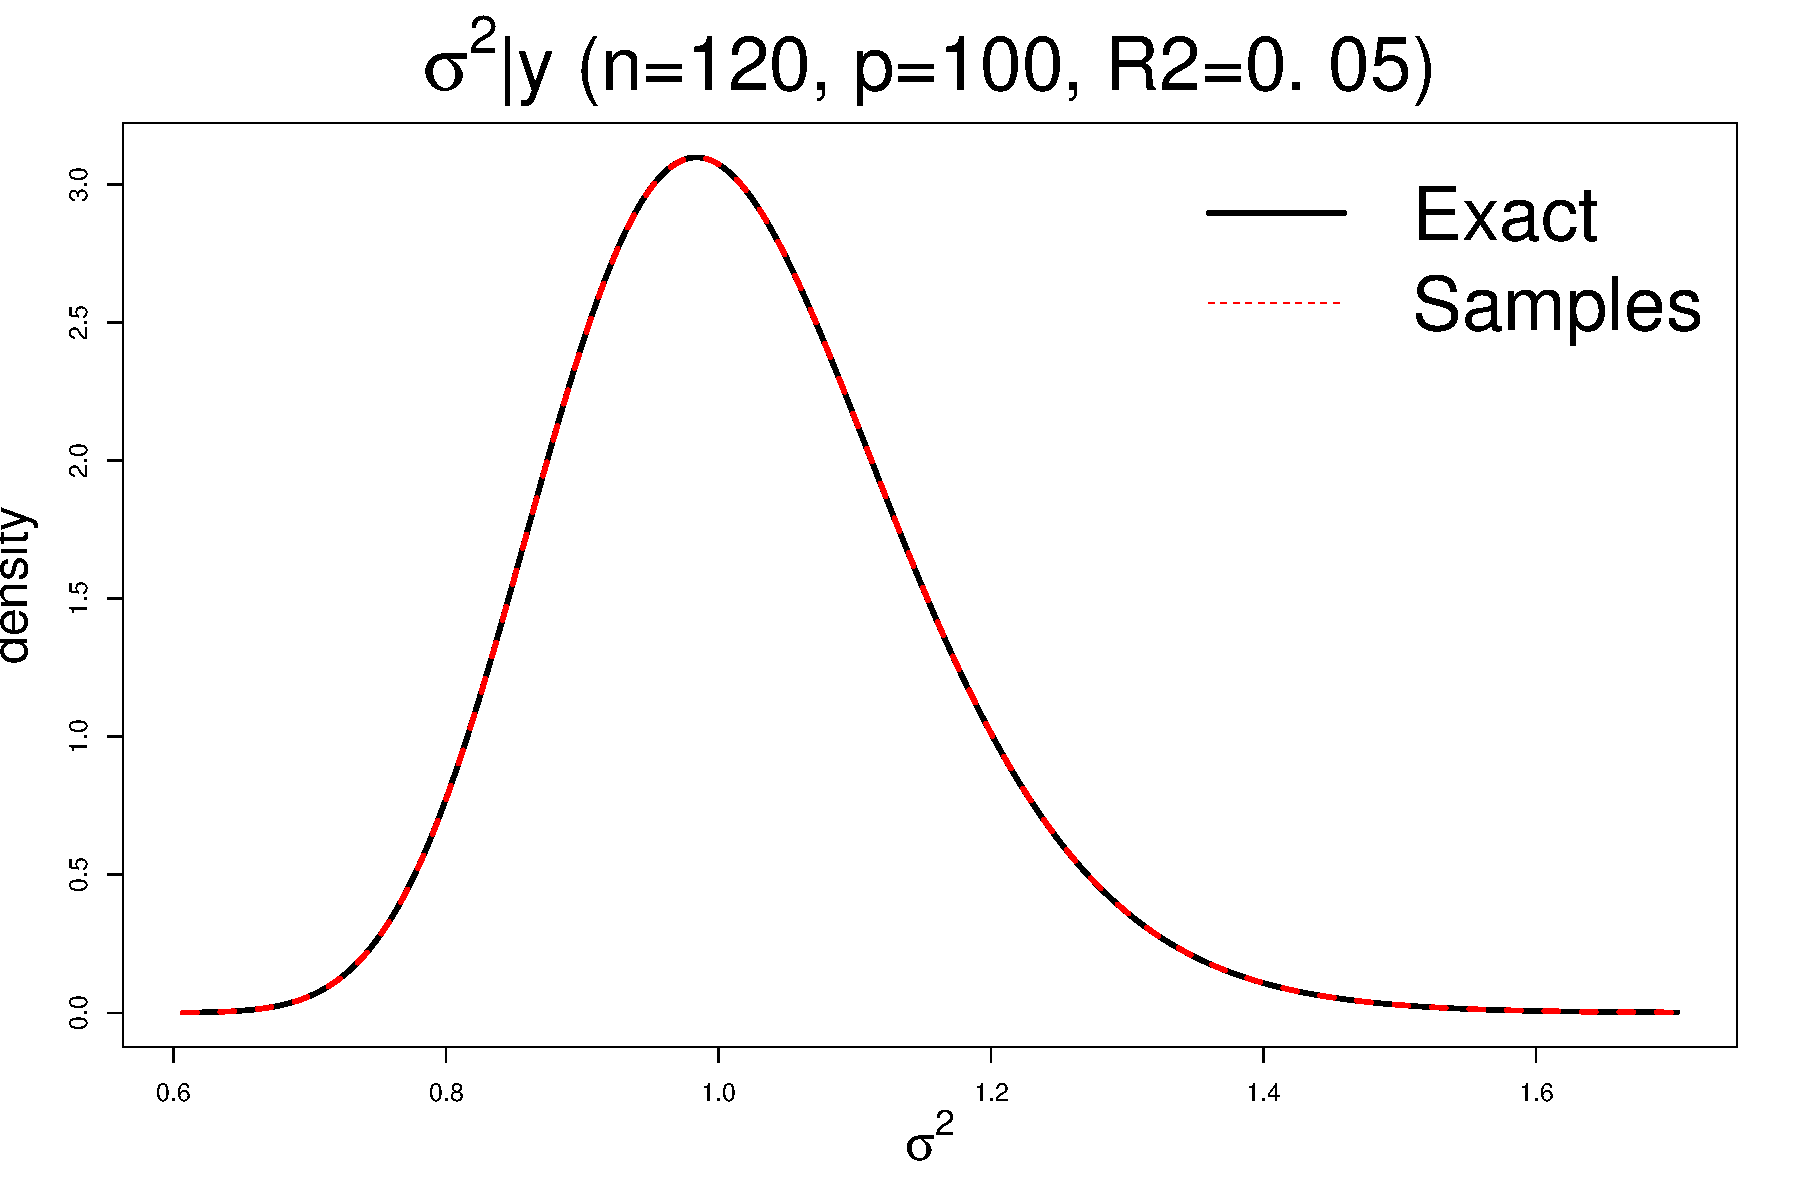
\includegraphics[width=.5\textwidth]{sigma2GivenY.pdf} \\
				% \caption{$g | \vy$}
				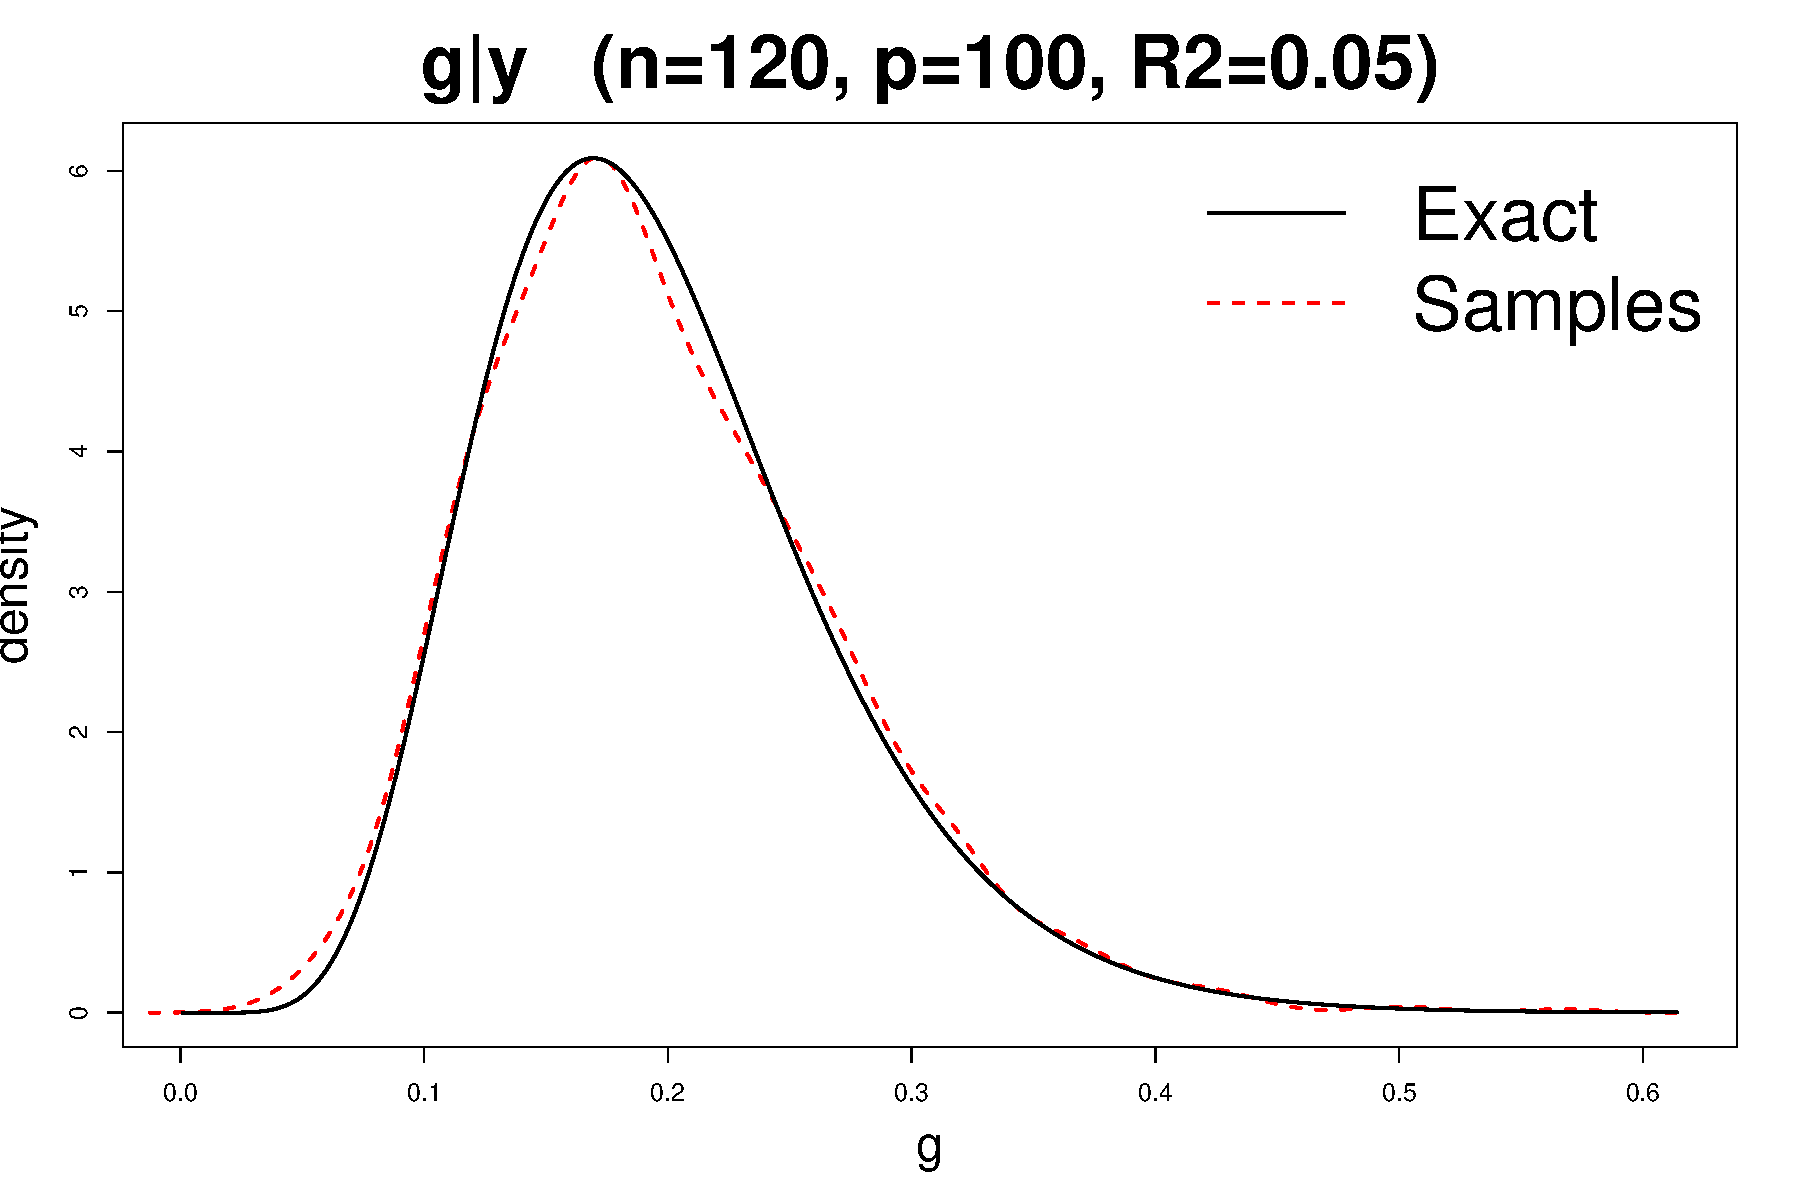
\includegraphics[width=.5\textwidth]{gGivenY.pdf} &
				% \caption{$\alpha | \vy$}
				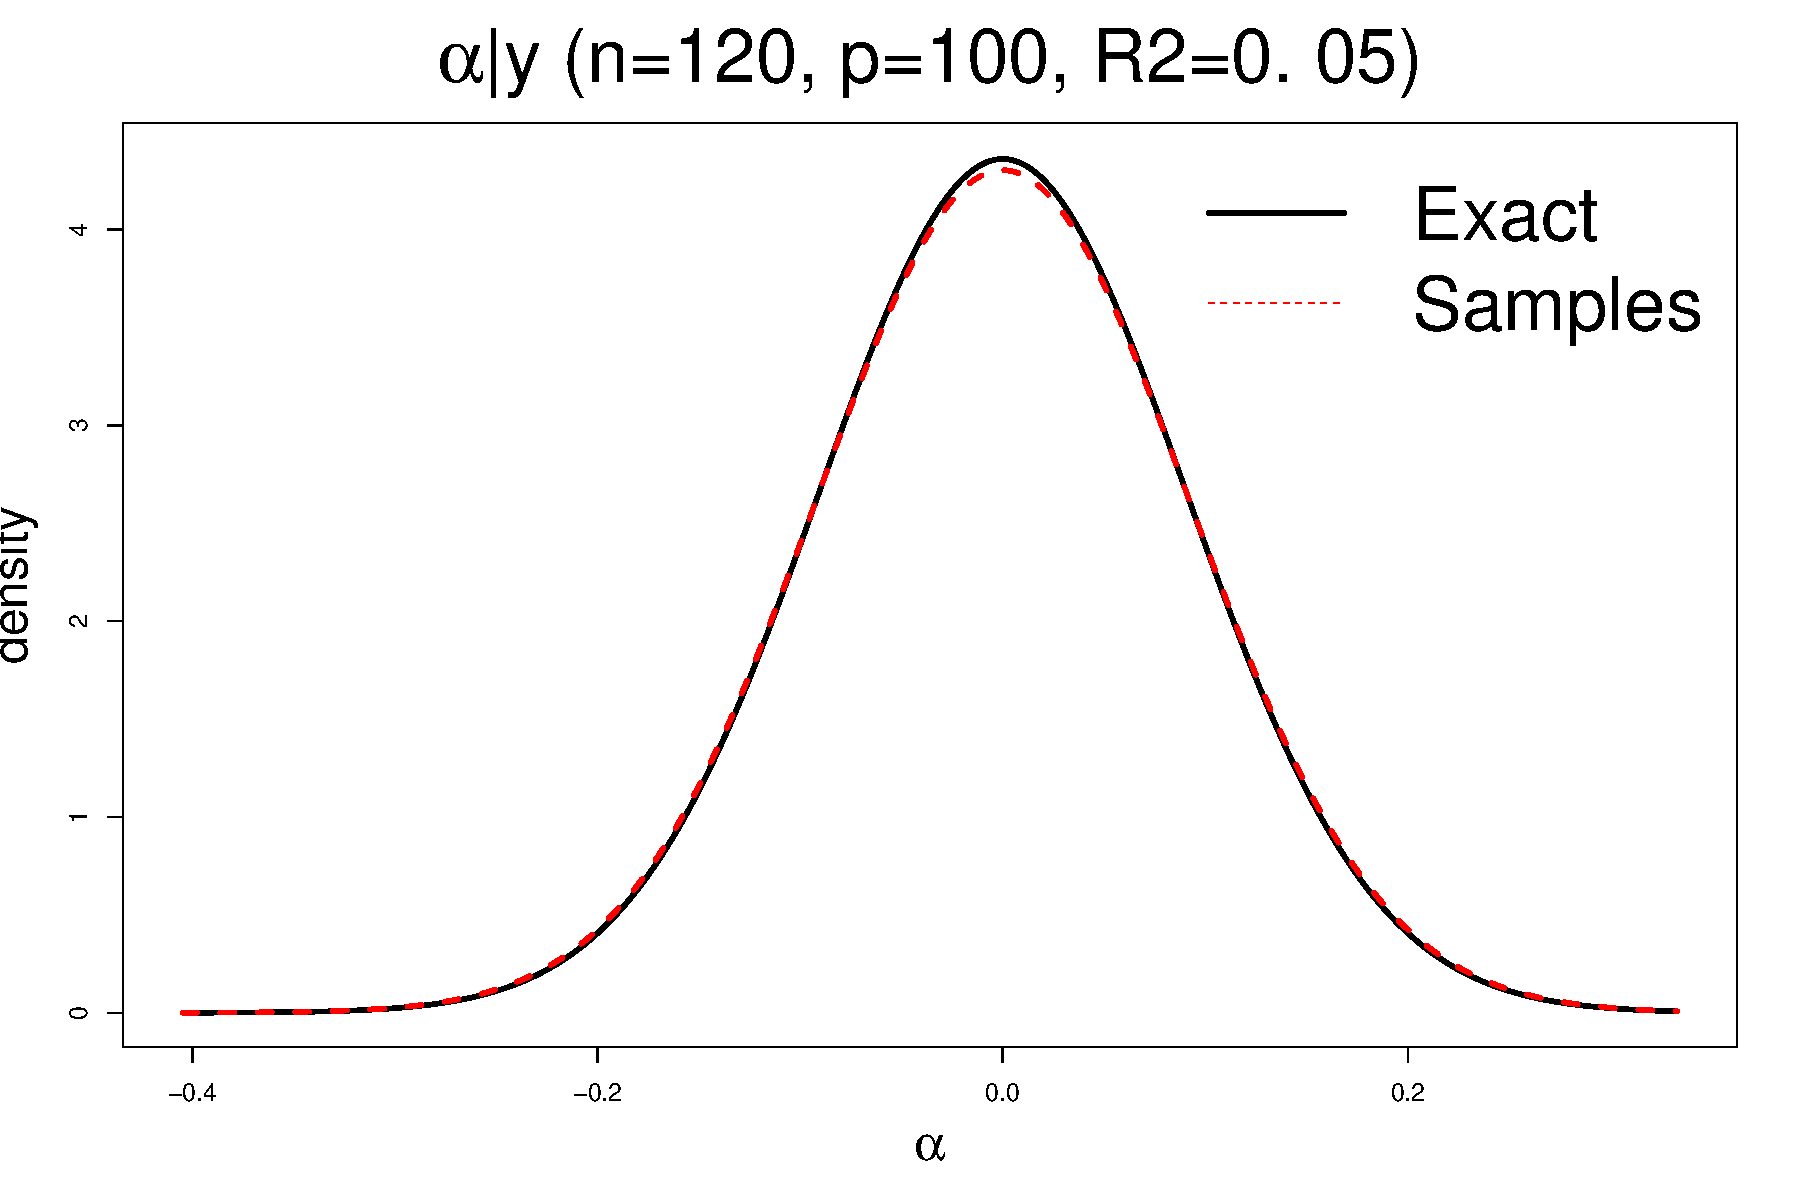
\includegraphics[width=.5\textwidth]{alphaGivenY.pdf}
			\end{array}$
		\end{center}
		\includegraphics[width=.5\textwidth]{uGivenY.pdf}
		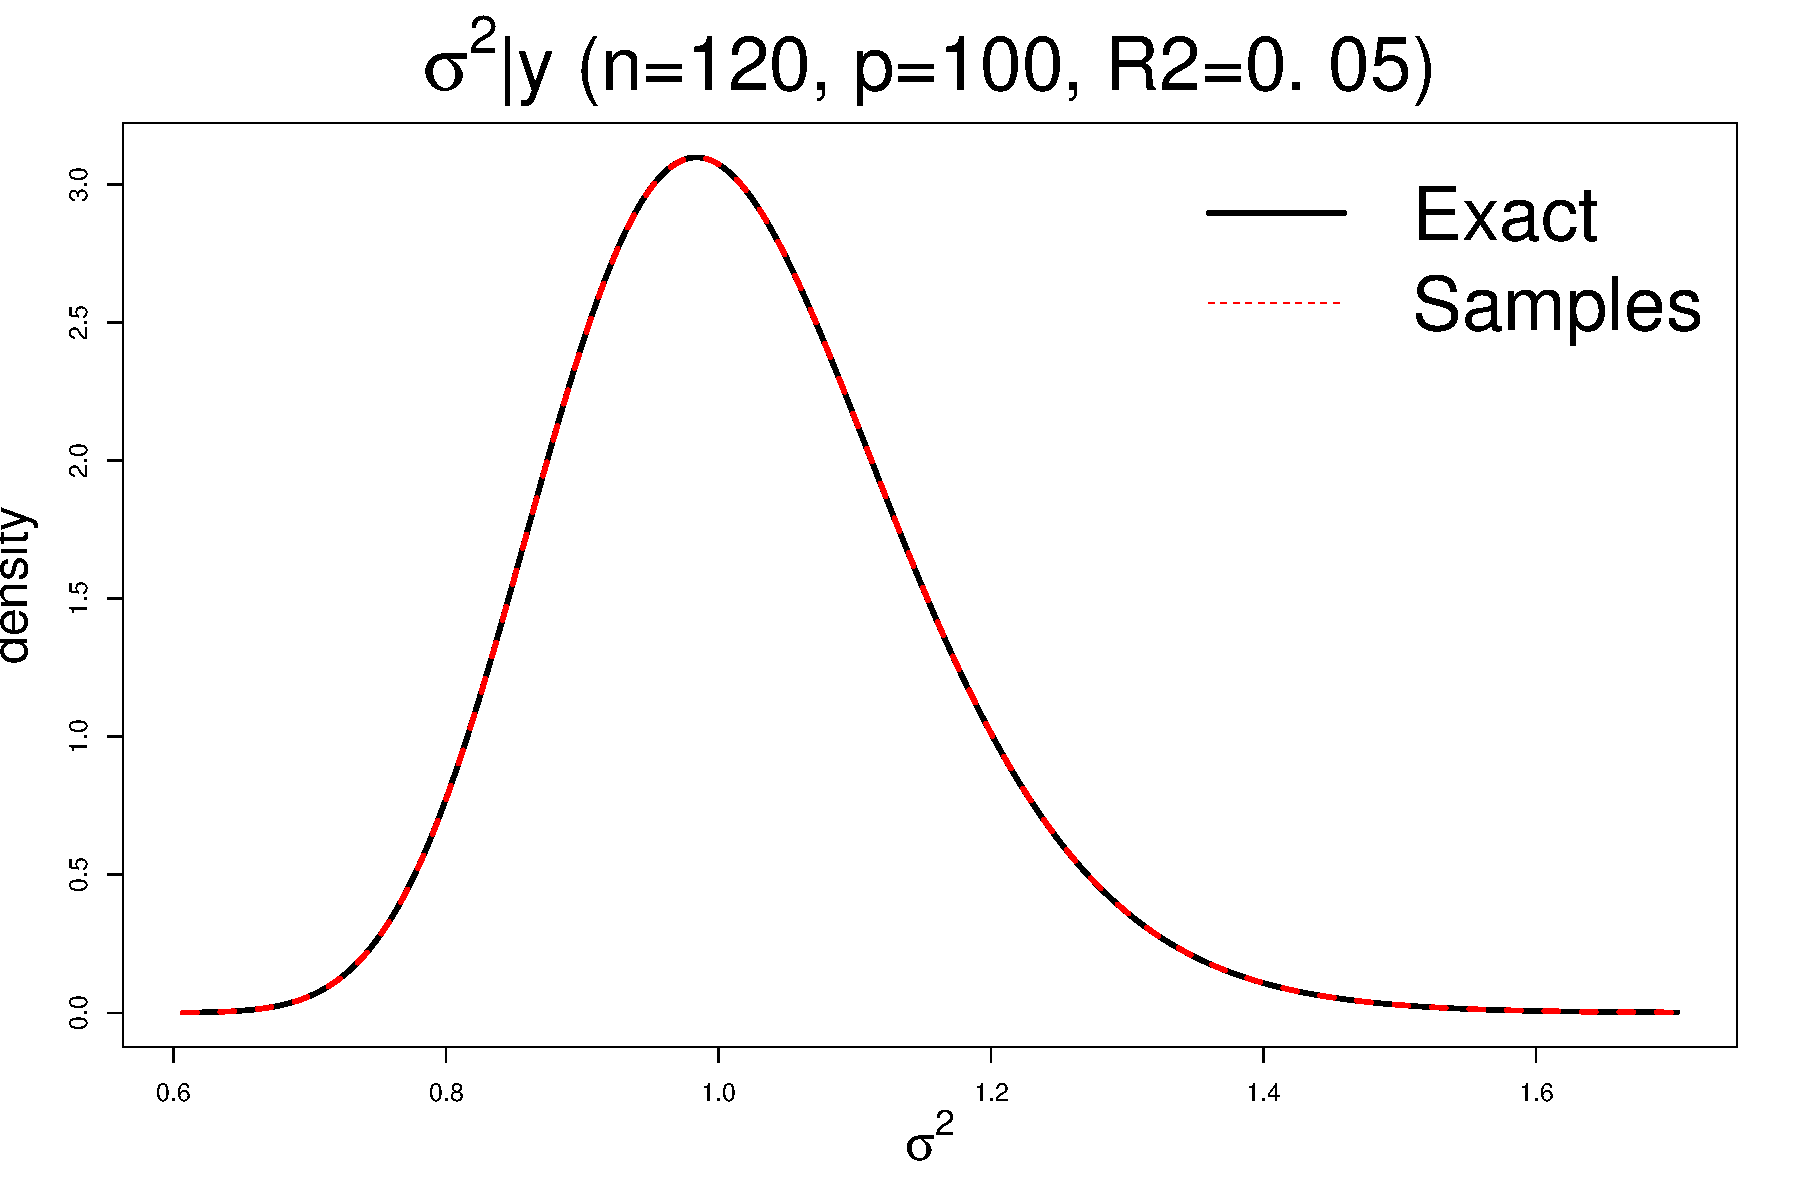
\includegraphics[width=.5\textwidth]{sigma2GivenY.pdf}
		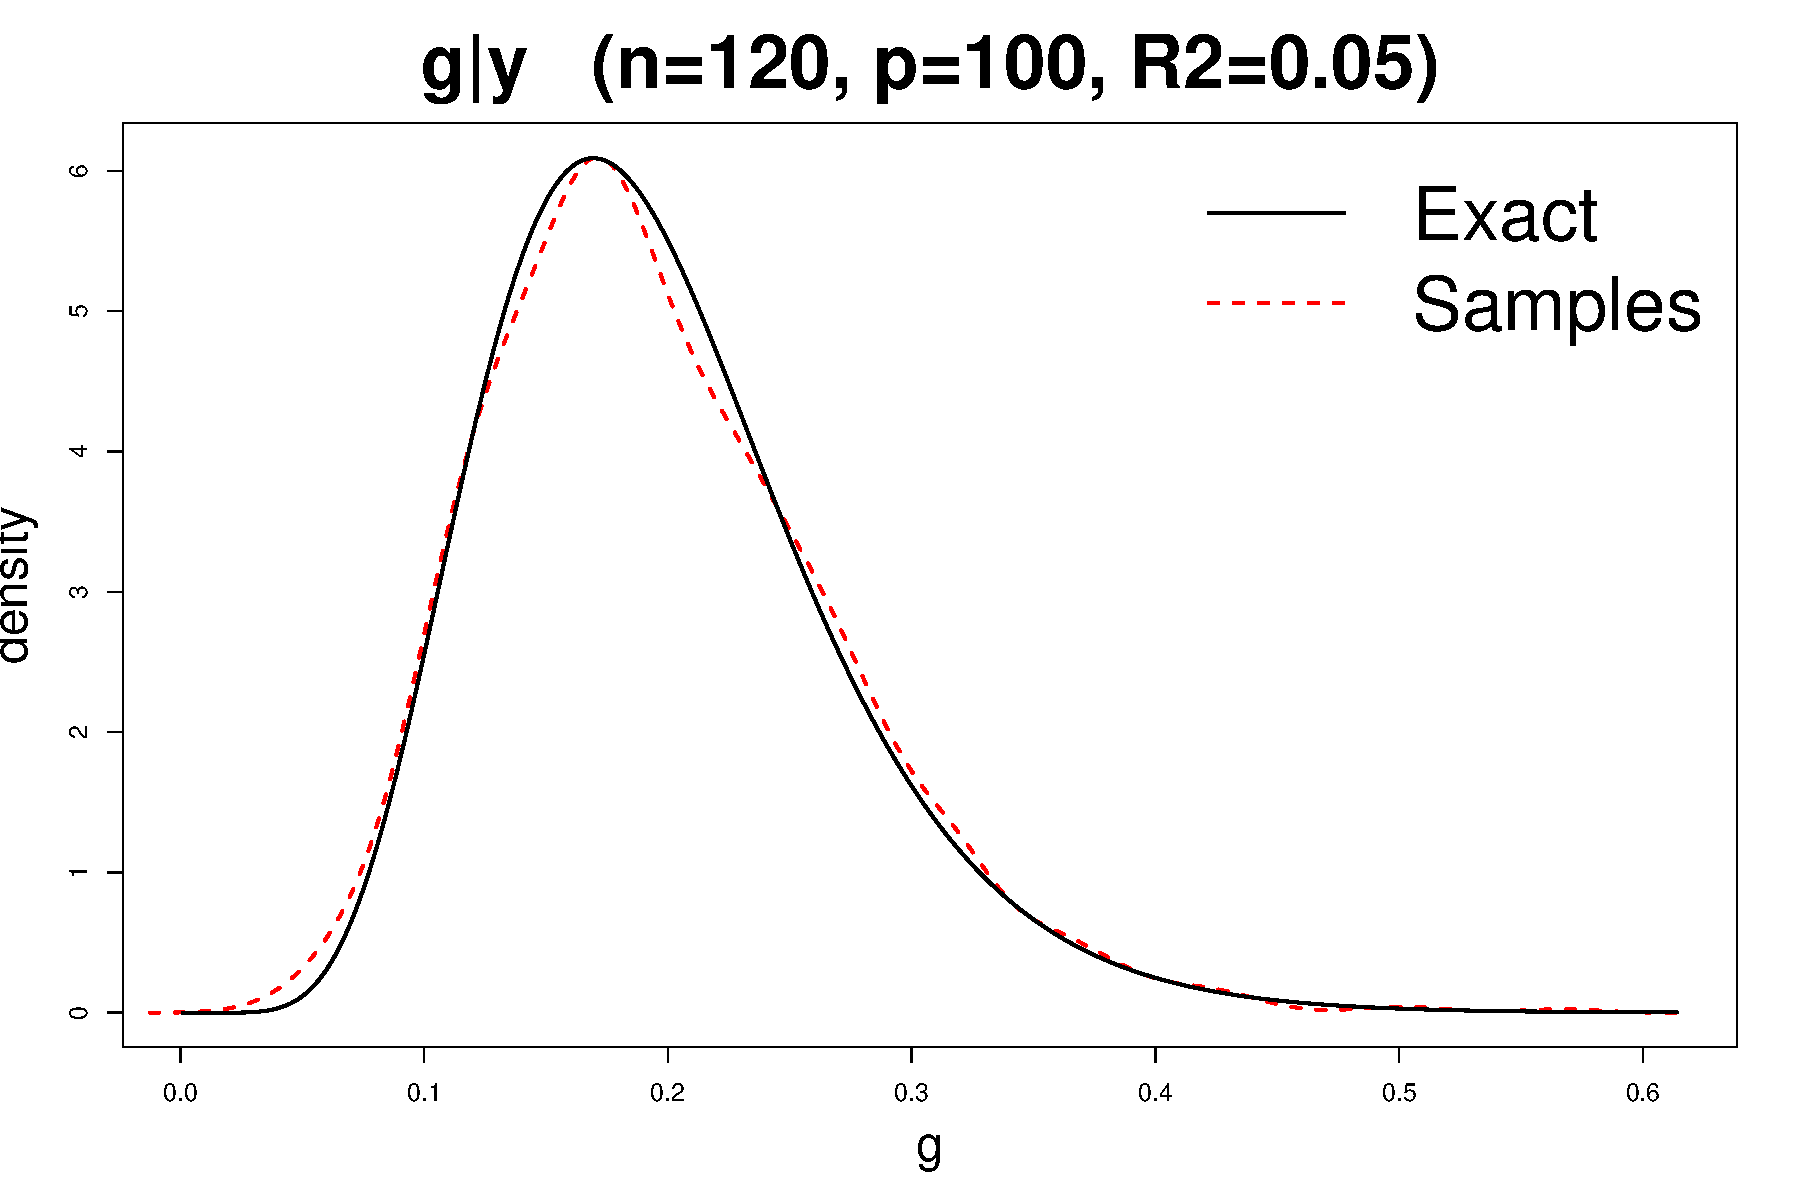
\includegraphics[width=.5\textwidth]{gGivenY.pdf}
		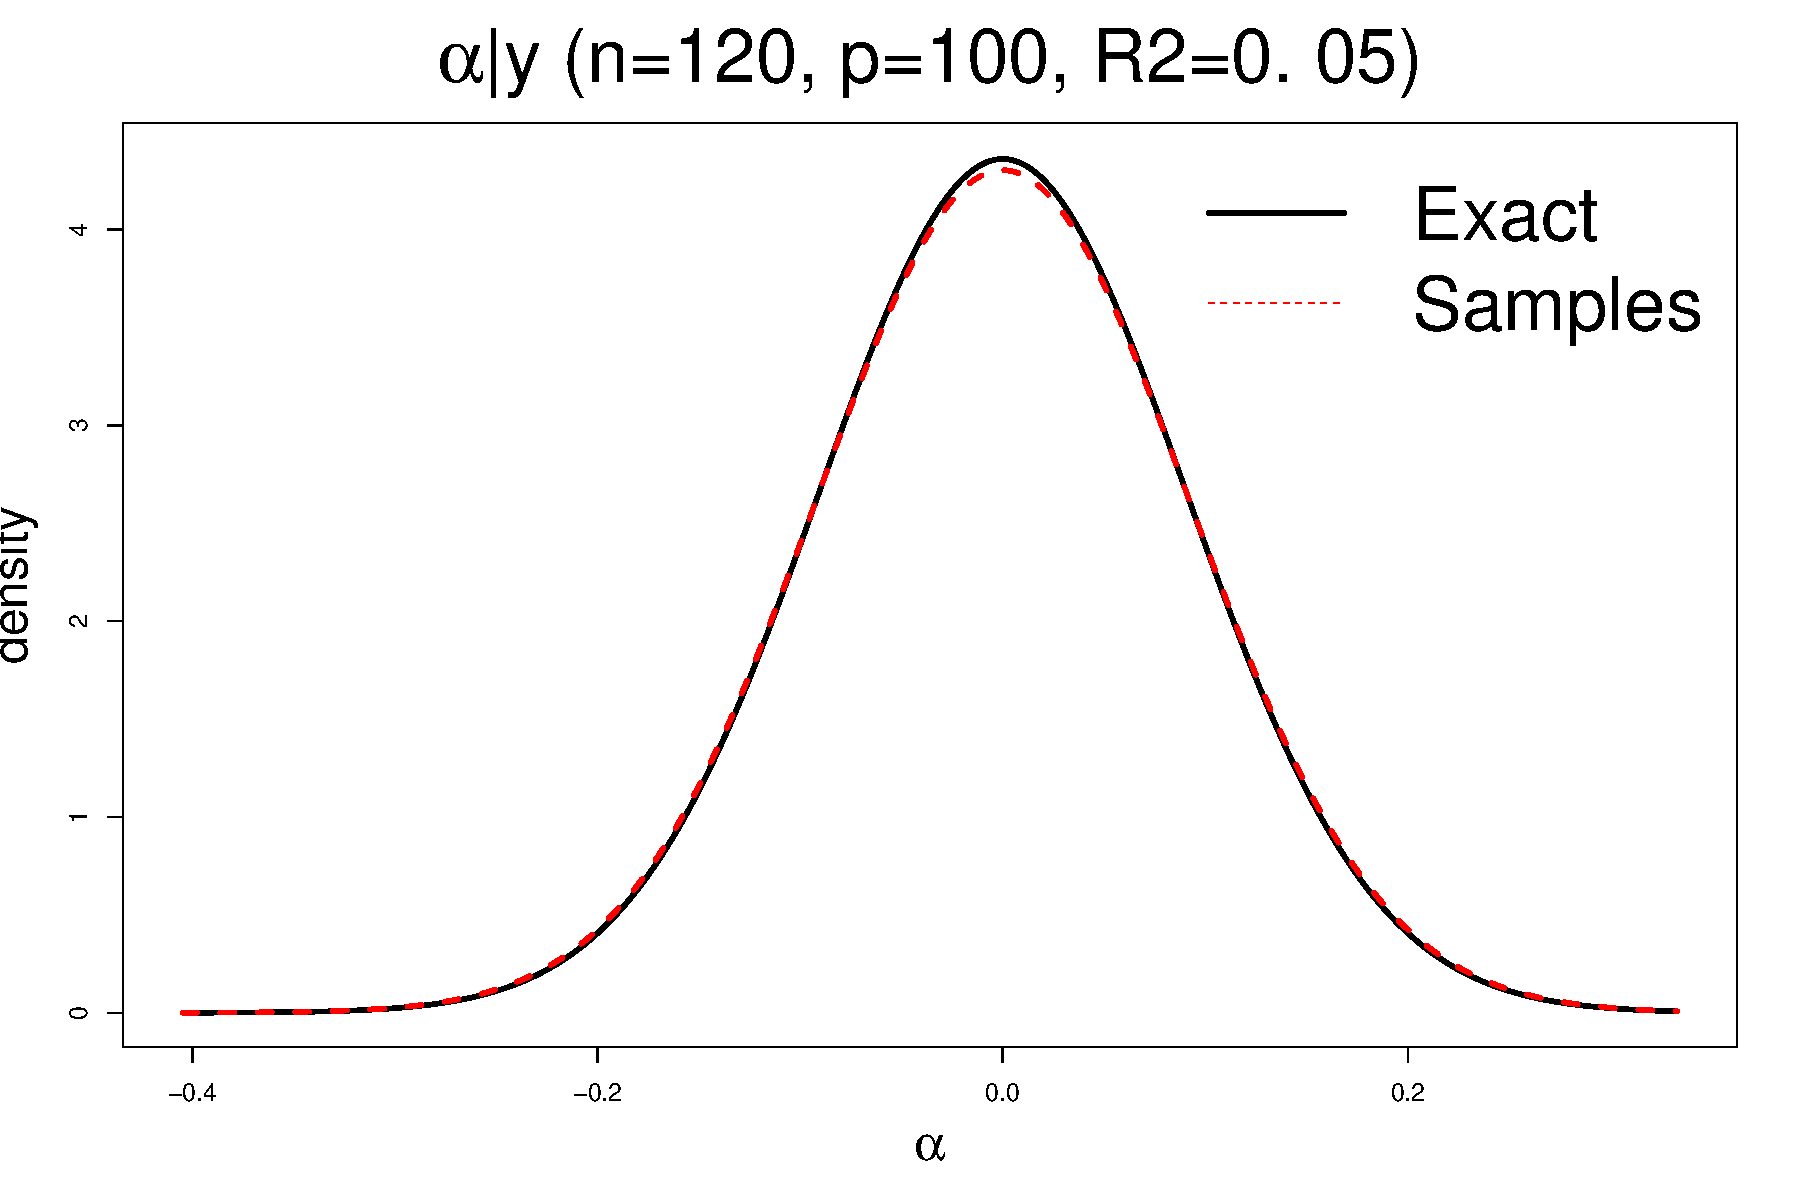
\includegraphics[width=.5\textwidth]{alphaGivenY.pdf}
	\end{figure}
\end{frame}

\begin{frame}
	\frametitle{Application: US Crime data}
	\begin{figure}
		\caption{Example model fit to the US Crime data}
		\includegraphics[scale=.33]{BetaUSCrime.pdf}
	\end{figure}
\end{frame}

\begin{frame}
	\frametitle{References / Contact details}
	\begin{itemize}
		\item Mark Greenaway
		\item markg@maths.usyd.edu.au
		\item Twitter: @certifiedwaif	
	\end{itemize}

	\small
	\bibliographystyle{elsarticle-harv}
	\bibliography{../references_mendeley}
\end{frame}

\end{document}
